\documentclass[a4paper,10pt]{article}
\usepackage[utf8]{inputenc}

\usepackage[english]{babel}
\usepackage[dvinames]{xcolor}
\usepackage[compact,small]{titlesec}
\usepackage{booktabs}
\usepackage{multirow}
\usepackage{amsfonts,amsmath,amssymb}
\usepackage{marginnote}
\usepackage[top=1.8cm, bottom=1.8cm, outer=1.8cm, inner=1.8cm, heightrounded, marginparwidth=2.5cm, marginparsep=0.5cm]{geometry}
\usepackage{enumitem}
\setlist{noitemsep,parsep=2pt}
\newcommand{\highlight}[1]{\textcolor{kuleuven}{#1}}
%\usepackage{pythonhighlight}
\usepackage{cleveref}
\usepackage{graphicx}
\usepackage{subfigure}
\usepackage{float}


\newcommand{\nextyear}{\advance\year by 1 \the\year\advance\year by -1}
\newcommand{\thisyear}{\the\year}
\newcommand{\deadlineGroup}{November 27, \thisyear{} at 16:00 CET}
\newcommand{\deadlineCode}{December 18, \thisyear{} at 16:00 CET}
\newcommand{\deadlineReport}{January 4, \nextyear{} at 16:00 CET}

\newcommand{\ReplaceMe}[1]{{\color{blue}#1}}
\newcommand{\RemoveMe}[1]{{\color{purple}#1}}

\setlength{\parskip}{5pt}

%opening
\title{Evolutionary Algorithms: Final report}
\author{Georgios Kouros (r0816917)}

\begin{document}
\fontfamily{ppl}
\selectfont{}

\maketitle

\section{Metadata}

\begin{itemize}
 \item \textbf{Group members during group phase:} Kostantinos Gkentsidis and Jeffrey Quicken
 \item \textbf{Time spent on group phase:} 20 hours
 \item \textbf{Time spent on final code:} 30 hours
 \item \textbf{Time spent on final report:} 10 hours
\end{itemize}

\section{Modifications since the group phase}

%\RemoveMe{\textbf{Goal:} Based on this section, we will evaluate insofar as you are able to analyse common problems arising in the design and implementation of evolutionary algorithms and your ability to effectively solve them.}

\subsection{Main improvements}

%\ReplaceMe{List the main changes that you implemented since the group phase. You do not need to explain the employed techniques in detail; for this, you should refer to the appropriate subsection of section 3 of the report.}

%\paragraph{} \ReplaceMe{Short description 1: State what modification you made (e.g., replaced top-$\lambda$ selection with $k$-tournament selection). What aspect of your evolutionary algorithm did it improve?} 

\paragraph{Greedy Heuristic Initialization}: Added a heuristic initialization of candidate solutions in order to inject some good initial candidates to the random initial population and speed up the search of the optimum.

\paragraph{Local Search:} Converted the evolutionary algorithm to a memetic algorithm through the inclusion of 2-opt/3-opt local search after the variation step of each iteration. This addition significantly improved convergence to really good candidate solutions.

\paragraph{Mutation Self-Adaptivity:} Self-adaptivity was added to vary mutation rate and strength in order to improve the diversity of the population across iterations and prevent premature convergence.

\paragraph{Diversity Promotion}: Fitness sharing was added to the $(\lambda+\mu)$~elimination step to improve the diversity of the population across iterations and prevent premature convergence.


\subsection{Issues resolved}
%\ReplaceMe{Recall the list of issues from the group phase. Describe how you solved these issues in the individual phase.}

%\paragraph{}\ReplaceMe{Short description 1: Describe the observation or problem from the group phase. Explain what caused this issue. How did you solve it (you can refer to the list of improvements)? Did fixing it significantly benefit your evolutionary algorithm? If you did not fix it: why not?}

\paragraph{Depleting Diversity:} In the group phase, we detected a problem with diversity, meaning that our algorithm converged prematurely to locally optimal candidate solutions, thus preventing the discovery of better solutions. This issue was fixed through the addition of diversity promotion schemes, namely fitness-sharing elimination and self-adaptive mutation rate and strength.

\paragraph{Premature convergence:} In the group phase, we used the $(\lambda+\mu)-elimination$ in combination with a convergence criterion of matching mean to best fitness. This resulted in a mostly exploitative behavior resulting in premature convergence. This issue was fixed by implementing methods for diversity promotion.

\paragraph{Loss of Best Candidate:} In the individual phase it was discovered that sometimes the best candidate was lost across iterations. This was easily visible as unexplained spikes in the corresponding graph across iterations. This happened due to an unwanted modification of the original population during mutation. Fixing this bug cleared this error.

\paragraph{Inefficient Crossover Operator:} The code used for the Order Crossover operator was taken from stackoverflow. In an effort to refine this code and remove needless code repetition, the operator was written from scratch and ended up being more efficient, shorter and more readable.

\section{Final design of the evolutionary algorithm} 

%\RemoveMe{\textbf{Goal:} Based on this section, we will evaluate insofar as you are able to design and implement an advanced, effective evolutionary algorithm for solving a model problem.}

%\ReplaceMe{In this section, you should describe all components of your final evolutionary algorithm and how they fit together.}

\subsection{Representation}

%\ReplaceMe{How do you represent the candidate solutions? What is your motivation to choose this one? What other options did you consider? How did you implement this specifically in Python (e.g., a list, set, numpy array, etc)?}

The authors in ~\cite{davis} present five different representations for TSP: Binary, Path, Adjacency, Ordinal, and Matrix representations. Based on a review of the different methods in the same research, it was decided in the group phase to select the \textbf{Path} / \textbf{Permutation Representation}, because of its better performance, operator variety, and explainability. The same representation was kept in the individual phase. This  Path representation was implemented as a python class called Individual that stores a list of integers representing indices of cities with respect to the given distance matrix. The route of the candidate solution is checked against errors on update and hence the use of python sets was deemed redundant.
\subsection{Initialization}

%\ReplaceMe{How do you initialize the population? How did you determine the number of individuals? Did you implement advanced initialization mechanisms (local search operators, heuristic solutions)? If so, describe them. Do you believe your approach maintains sufficient diversity? How do you ensure that your population enrichment scheme does not immediately take over the population? Did you implement other initialization schemes that did not make it to the final version? Why did you discard them? How did you determine the population size?}

In the group phase, a random initialization was used for the population resulting in high diversity with a high probability given a big enough population size $\lambda$. In order to achieve good results, it was decided to use a quite large population (1000-2000).

In the individual phase, the initialization step was augmented with a number (eg. 10) of greedy heuristic candidate solutions in order to provide some direction to the search and avoid reinventing the wheel. The greedy heuristic search starts from a random city keeps following the shortest path from city to city until all cities are visited only once and finally ends up on the first city.  

The use of really good candidate solutions entails the danger of taking over the population fairly quickly. However, this issue can be mitigated by limiting the steps of the greedy search, although, because of the implemented diversity promotion schemes, it was not deemed necessary.

Furthermore, the addition local search and diversity promotion, allowed the use of a population size that's one magnitude smaller $(\lambda = 100)$. Using a lower population size resulted in better performance and more iterations, while no severe impact was noted on the final results.

\subsection{Selection operators}

%\ReplaceMe{Which selection operators did you implement? If they are not from the slides, describe them. Can you motivate why you chose this one? Are there parameters that need to be chosen? Did you use an advanced scheme to vary these parameters throughout the iterations? Did you try other selection operators not included in the final version? Why did you discard them?}
Similarly to the group phase, k-tournament selection was picked for the individual phase as well. This selection method performed really well before and offered a nice balance between exploration and exploitation, hence it was decided to keep it.

The only tunable parameter of this selection operator is the number $k$ of individuals that take part in a tournament. During the tuning phase of the group phase a $k = 4$ was selected because of the good balance between convergence, exploration, and computational efficiency.

\subsection{Mutation operators} \label{ss_mut}

%\ReplaceMe{Which mutation operators did you implement? If they are not from the slides, describe them. How do you choose among several mutation operators? Do you believe it will introduce sufficient randomness? Can that be controlled with parameters? Do you use self-adaptivity? Do you use any other advanced parameter control mechanisms (e.g., variable across iterations)? Did you try other mutation operators not included in the final version? Why did you discard them?}

In the group phase, we implemented two mutation operators for permutation-based problems, namely the swap and the mutation operator. Of the two, inversion mutation proved to produce better results, which was evident from a thorough literature review as well. The inversion mutation operator was chosen for the individual phase as well, since it was one of the best performing operators in the literature with regard to the TSP problem. Both mutation operators, however, were augmented with a new parameter called mutation strength $\sigma_m$, which, determines the number of successive applications of the operator on an individual.

The mutation rate and strength are initialized as $p_m=0.1$ and $\sigma_m=1$ and they are modified across iterations via an adaptive parameter control scheme with a view to keep diversity above a certain threshold. This approach was inspired from \cite{mut_adapt} and involves two steps.

\begin{enumerate}
\item Estimating the diversity $d$ of the current iteration of the algorithm as the normalized number of unique individual fitnesses.

\item Updating the mutation rate $p_m$ and strength $\sigma_m$ according Eq. \ref{adapt_eq}

\begin{equation} \label{adapt_eq}
p' = max(p_{min},~min(p_{max}, ~p (1 + \frac{\xi (d_t-d)}{d})))
\end{equation}
where $p'$, $p$, $p_{min}$, $p_{max}$ are the adapted value, previous value, lower bound, and upper bound of the parameter to self adapt. Moreover, $\xi$ is the control of the adaptivity, $d$ is the current diversity and $d_t$ is the desired diversity.

\end{enumerate}


\subsection{Recombination operators}

%\ReplaceMe{Which recombination operators did you implement? If they are not from the slides, describe them. How do you choose among several recombination operators? Why did you choose these ones specifically? Explain how you believe that these operators can produce offspring that combine the best features from their parents. How does your operator behave if there is little overlap between the parents? Can your recombination be controlled with parameters; what behavior do they change? Do you use self-adaptivity? Do you use any other advanced parameter control mechanisms (e.g., variable across iterations)? Did you try other recombination operators not included in the final version? Why did you discard them? Did you consider recombination with arity strictly greater than 2?}

In the individual phase, it was decided to reuse the \textit{Order Crossover} \cite{davis} operator, since it performs really well for order-based permutation problems like TSP according to the literature eg. \cite{memetic} and based on experiments. In addition, another advantage of this operator is that it ensures the generation of only valid offspring and thus doesn't require the need to implement a repair mechanism.

The only change regarding this operator was the rewritting of its code to make it more efficient and readable.

The operator consists of the following steps:
\begin{itemize}
\item Copy a segment between two randomly generated crossover points of the first parent to the first child.
\item Starting from the second crossover point on the second parent this time, start copying its genes/alleles that are not already contained on the child, until the child is full.
\item Create the second child like the first but with the reverse order of the parents.
\end{itemize}

The operator, in general, preserves a segment of the first parent on the child and then tries to fill the rest with the city order of the second parent, thus preserving useful information from both parents. At the same time, because of the combination of two random parents that may or may not have much overlap, the resulting children can be similar to the parents and explore new space, while always producing valid candidate solutions.

One enhancement that was considered was to add more recombination operators that vary significantly to Order Crossover and then have each individual randomly select its own, which would potentially result in greater exploration of the search space.

\subsection{Elimination operators} \label{ss_elim}

%\ReplaceMe{Which elimination operators did you implement? If they are not from the slides, describe them. Why did you select this one? Are there parameters that need to be chosen? Did you use an advanced scheme to vary these parameters throughout the iterations? Did you try other elimination operators not included in the final version? Why did you discard them?}

In the group phase, there was no choice but to use the $(\lambda+\mu)-elimination$ operator, which did not achieve a good balance between exploration and exploitation. This method chooses the top-$\lambda$ candidates and eliminates worse candidate solutions that could result in better results after a few generations. Instead it even promotes similar candidates that have high fitness, which often causes premature convergence.

In the individual phase, two more elimination operators were implemented, namely, \textit{fitness-sharing-based elimination} and \textit{replace-worst elimination}.

Fitness-sharing-based elimination is basically implemented as $(\lambda+\mu)-elimination$ with a recalculated fitness of each individual based on the number of its neighbouring individuals. This basically means that the fitness of similar individuals in the population is increased, so that more diverse individuals make it to the next generation. The best candidate solution of each generation is not weighted so that it's not eliminated.

Replace-worst elimination results in a more diverse population than the simple $(\lambda+\mu)-elimination$ by keeping the $\lambda-\mu$ best individuals from the original population and replacing the rest with new offspring. This requires that $\lambda > \mu$.

Out of all three, the fitness-sharing-based elimination achieved the best and most consistent results and prevented premature conversion. Although, one main problem with this method is that it invalidates the previously used convergence criteria, since it does not allow the mean fitness to converge to the best fitness.

\subsection{Local search operators}

%\ReplaceMe{What local search operators did you implement? Describe them. Did they cause a significant improvement in the performance of your algorithm? Why (not)? Did you consider other local search operators that did not make the cut? Why did you discard them? Are there parameters that need to be determined in your operator? Do you use an advanced scheme to determine them (e.g., adaptive or self-adaptive)?}
The absence of a local search operator in the group phase meant that the implemented evolutionary algorithm required a considerable amount of iterations or a really large population in order to find a good solution. As a result, it was deemed imperative to implement a local search operator for the individual phase. After a thorough literature review of the available methods, it was decided to proceed with k-opt local search, proposed by Croes et al \cite{k-opt}.

The local search operator was implemented for $k=2$ and $k=3$. However, the 3-opt operator proved quite inefficient especially for the larger problems and thus was abandoned in favor of 2-opt. A basic 2-opt local search algorithm will try all possible swap combinations that will result in an improvement of the fitness of an individual. If no more improvement can be made then it returns.

Although, 2-opt increases the computational complexity of the algorithm, at the same time, it results in quicker discovery of really good solutions. For really large problems, however, the operator proves extremely slow and thus a two-pronged approach has been implemented to optimize the evolutionary algorithm. Firstly, a new parameter has been introduced that determines the probability threshold $p_l$ for executing local search in a generation. Secondly, a timeout of one second has been added to the two-opt local operator. As a result, the operator will perform the maximum number of improvements it manages in the one second period.


\subsection{Diversity promotion mechanisms}

%\ReplaceMe{Did you implement a diversity promotion scheme? If yes, which one? If no, why not? Describe the mechanism you implemented. In what sense does the mechanism improve the performance of your evolutionary algorithm? Are there parameters that need to be determined? Did you use an advanced scheme to determine them?}

In the individual phase, two diversity promotion mechanisms were implemented. The first one involves a varying mutation rate and strength, which was described in detail in Subsection \ref{ss_mut}. The second one is fitness sharing, it is implemented in the elimination step and it's described in more detail in Subsection \ref{ss_elim}.

There is no point in using both mechanisms at the same time, since the adaptive control of the mutation parameters activates when diversity lowers below a threshold, which doesn't happen when fitness sharing is active.

The fitness sharing mechanism has two tunable parameters $\alpha$ and $\sigma$ that determine its sensitivity. A larger $\alpha$ value results in a higher penalty for each neighbour and $\sigma$ represents the distance between two individuals for them to be considered neighbours. 

\subsection{Stopping criterion}

%\ReplaceMe{Which stopping criterion did you implement? Did you combine several criteria?}

In the individual phase, two convergence criteria were used. The first one was the same that was used in the group phase. This criterion ended the algorithm when the mean fitness converged to the best fitness of the population. However, because of the diversity promotion mechanisms that were implemented, this criterion was replaced by a new one that simply checkeq if there was no improvement of the best fitness in $30\%$ of the past iterations, provided that at least $N=20$ iterations had passed.

\subsection{The main loop}

%\ReplaceMe{Describe the main loop of your evolutionary algorithm using a clear picture (preferred) or high-level pseudocode. In what order do you apply the various operators? Why that order? If you are using several selection, mutation, recombination, elimination, and local search operators, describe how you choose among the possibilities. Are you selecting/eliminating all individuals in parallel, or one by one? With or without replacement?}

\begin{center}
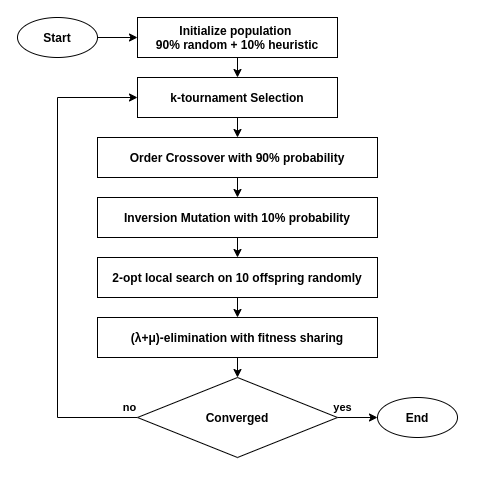
\includegraphics[scale=0.7]{images/genetic_algorthm_main_loop.png} 
\end{center}

In each generation, for each offspring pair, two parents are selected that will produce the offspring pair using recombination with $90\%$ probability. If recombination fails, then the parents are passed to the next step. This step involves inversion mutation with $10\%$ probaility. If this step fails as well, then the offspring are the same as the parents. After all offspring have been generated for a single generation, a 2-opt local search mechanism attempts to optimize those offspring. Finally, a $(\lambda+\mu)-elimination$ method selects the new population by combining the old population with the new offspring, sorting the combined population and keeping the $top-\lambda$ individuals. Since, we use fitness sharing however, after the new population has been selected, each individual in the new population is re-weighted according to its similarity with other individuals, in order to limit the survivability of multiple similar good candidates. That's also one reason why elimination is done without replacement.

Selection is done with replacement, so that there is increased probability to pick really good individuals multiple times to recombine with other individuals. We basically desire good genes to propagate inside the population.

\subsection{Parameter selection}

%\ReplaceMe{For all of the parameters that are not automatically determined by adaptivity or self-adaptivity (as you have described above), describe how you determined them. Did you perform a hyperparameter search? How did you do this? How did you determine these parameters would be valid both for small and large problem instances?}

The main parameters that were tuned in the group phase were the population size, offspring size, mutation rate, k of k-tournament selection, as well as mutation rate and recombination rate. Since, good values for those parameters is already known, only minimal effort was done to tune them. Most of the tuning effort was focust on the new hyperparameters that were introduced in the individual phase.

Because of the addition of local search and fitness sharing, the algorithm grew more computationally expensive. As a result the population size and the offspring size were significantly reduced by an order of magnitude to allow the algorithm to run for more generations before time runs out. In particular, $\lambda$ was reduced from $2000$ to $100$ and $\mu$ was reduced from around $2000/3$ to $20$.

One of the biggest bottlenecks of the algorithm is 2-opt local search. As a result it was decided that local search will be applied in a generation with a probability $p_l$. This probability was tuned through  hyperparameter search. In Figure \ref{fig;prob-ls} there is a graph demonstrating the best fitness that the algorithm achieves for various local search probability values ranging from $0.0$ to $1.0$. Furthermore, Figure \ref{fig:prob-ls}, also displays the number of iterations that the algorithm run for, for each $p_l$ value. Based on those graphs we can safely pick $p_l = 0.3$, ensuring both efficiency and finding a good solution. 

\begin{figure}[H]
    \centering
	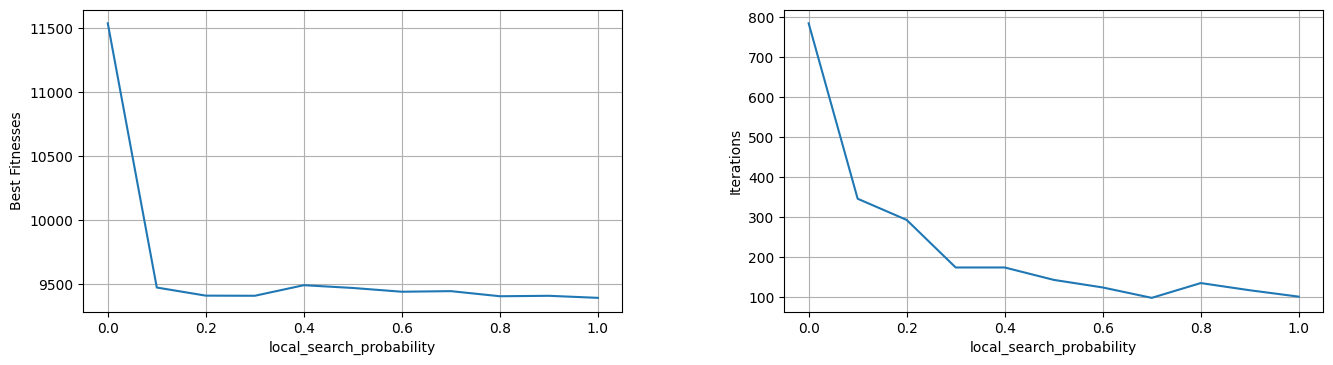
\includegraphics[width=\textwidth]{results/tuning/prob_LS.png}
    \caption{Best Fitness and Number of Iterations for various local search probability values}
    \label{fig:prob-ls}
\end{figure}

Another parameter that was added in the individual phase is the mutation strength $\sigma_m$, which was also tuned via hyperparameter search. The results are shown in Figure \ref{fig:sigma-mu}. The algorithm achieved the best results for $\sigma_m = 3$, although, it could just be a matter of luck. A more thorough hyperparameter search would repeatedly run the same experiment and then decide the best value based on the mean of the results. 

\begin{figure}[H]
    \centering
	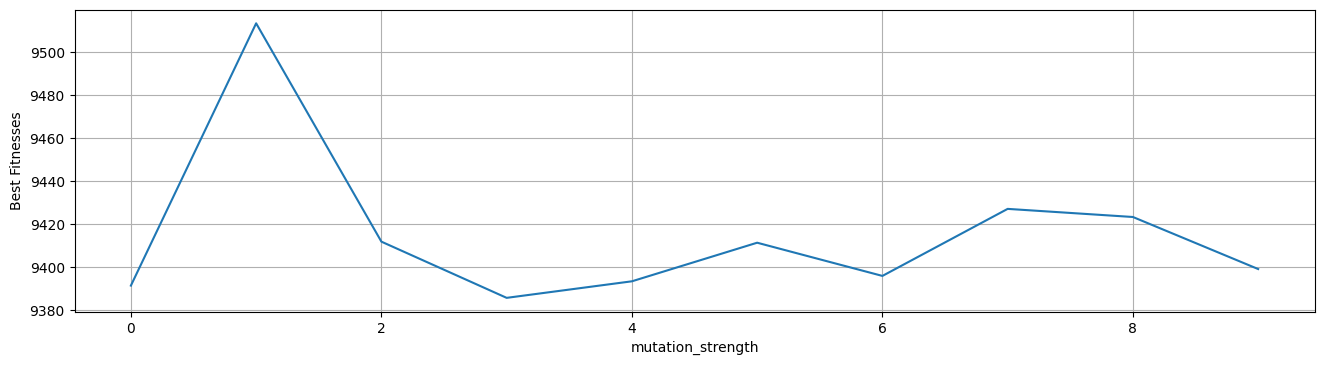
\includegraphics[width=\textwidth]{results/tuning/sigma_mu.png}
    \caption{Best Fitness for various mutation strength values}
    \label{fig:sigma-mu}
\end{figure}

%\subsection{Other considerations}

%\ReplaceMe{Did you consider other items not listed above, such as elitism, multiobjective optimization strategies (e.g., island model, pareto front approximation), a parallel implementation, or other interesting computational optimizations (e.g. using advanced algorithms or data structures)? You can describe them here or add additional subsections as needed.}


\section{Numerical experiments}

%\RemoveMe{\textbf{Goal:} Based on this section and our execution of your code, we will evaluate the performance (time, quality of solutions) of your implementation and your ability to interpret and explain the results on benchmark problems.}

\subsection{Metadata}

\ReplaceMe{What parameters are there to choose in your evolutionary algorithm? Which fixed parameter values did you use for all experiments below? If some parameters are determined based on information from the problem instance (e.g., number of cities), also report their specific values for the problems below.

Report the main characteristics of the computer system on which you ran your evolutionary algorithm. Include the processor or CPU (including the number of cores and clock speed), the amount of main memory, and the version of Python 3.}

The following list presents the different parameters that were chosen for the experiments presented in the following subsections. 
\begin{itemize}
\item $\lambda = 100$: size of population
\item $\mu = 20$: size of offspring
\item $k = 4$: number of individuals in the k-tournament selection
\item $p_c = 0.9$: recombination probability per generation
\item $p_m = 0.1$: mutation probability per generation
\item $p_l = 0.3$: local search probabiility per generation
\item $\sigma_m = 3$: mutation strength
\end{itemize}

All experiments were run in a laptop with an Intel i7 processor with 4 physical cores, 8 logical cores, 8GB Ram, and a clock speed of 1.3GHz (3.9GHz turbo speed). No parallelization was used, so execution was limited to one core. Finally, all experiments were run with \textit{Python 3.8.5}.

\subsection{tour29.csv}



\ReplaceMe{Run your algorithm on this benchmark problem (with the 5 minute time limit from the Reporter). Include a typical convergence graph, by plotting the mean and best objective values in function of the time (for example based on the output of the Reporter class). 

What is the best tour length you found? What is the corresponding sequence of cities? 

Interpret your results. How do you rate the performance of your algorithm (time, memory, speed of convergence, diversity of population, quality of the best solution, etc)? Is your solution close to the optimal one?

Solve this problem 1000 times and record the results. Make a histogram of the final mean fitnessess and the final best fitnesses of the 1000 runs. Comment on this figure: is there a lot of variability in the results, what are the means and the standard deviations?}

\begin{figure}[H]
    \centering
	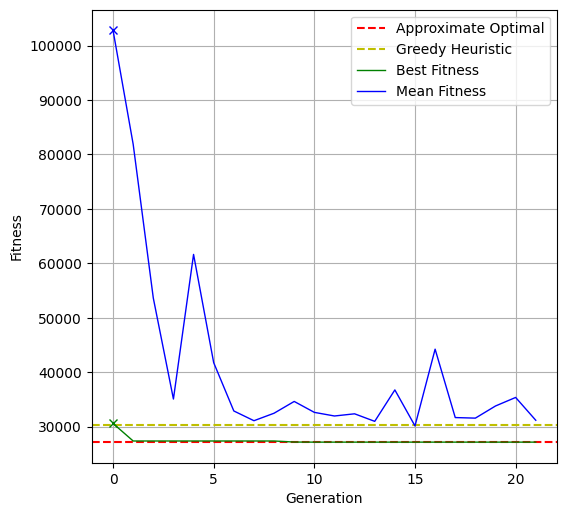
\includegraphics[width=0.5\textwidth]{results/4.2/tour29_convergence.png}
    \caption{Tour29 Convergence Graph}
    \label{fig:tour29convergence}
\end{figure}

\begin{figure}[H]
     \centering
     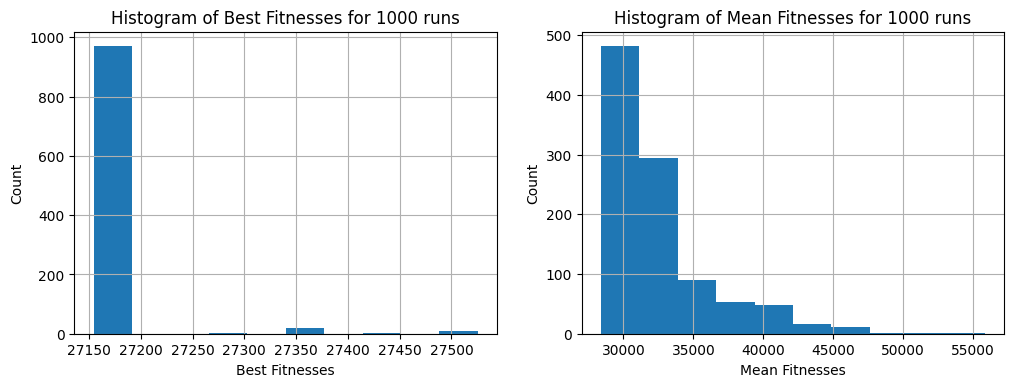
\includegraphics[width=\textwidth]{results/4.2/tour29_histogram.png}
     \caption{Tour29 1000 Run Histograms of Best and Mean Fitness}
     \label{fig:tour29histogram}
\end{figure}

\ReplaceMe{TODO add explanation} Figures \ref{fig:tour29convergence},  \ref{fig:tour29histogram}


\subsection{tour100.csv}

\ReplaceMe{Run your algorithm on this benchmark problem (with the 5 minute time limit from the Reporter). Include a typical convergence graph, by plotting the mean and best objective values in function of the time (for example based on the output of the Reporter class). 

What is the best tour length you found in each case? 

Interpret your results. How do you rate the performance of your algorithm (time, memory, speed of convergence, diversity of population, quality of the best solution, etc)? Is your solution close to the optimal one?}

\begin{figure}[H]
    \centering
	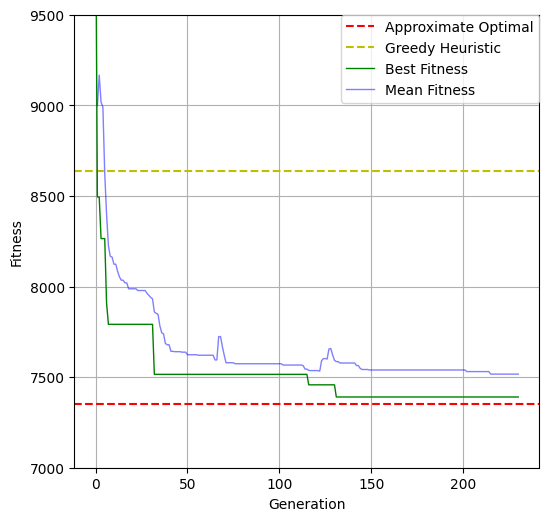
\includegraphics[width=0.5\textwidth]{results/4.3/tour100_convergence.png}
    \caption{Tour100 Convergence Graph}
    \label{fig:tour100convergence}
\end{figure}

\ReplaceMe{TODO add explanation} Figure \ref{fig:tour100convergence}

\subsection{tour194.csv}

\ReplaceMe{Run your algorithm on this benchmark problem (with the 5 minute time limit from the Reporter). Include a typical convergence graph, by plotting the mean and best objective values in function of the time (for example based on the output of the Reporter class). 

What is the best tour length you found? 

Interpret your results. How do you rate the performance of your algorithm (time, memory, speed of convergence, diversity of population, quality of the best solution, etc)? Is your solution close to the optimal one?}

\begin{figure}[H]
    \centering
	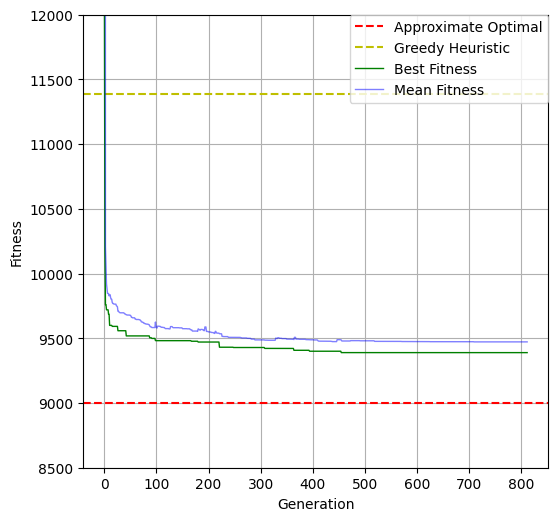
\includegraphics[width=0.5\textwidth]{results/4.4/tour194_convergence.png}
    \caption{Tour194 Convergence Graph}
    \label{fig:tour194convergence}
\end{figure}

\ReplaceMe{TODO add explanation} Figure \ref{fig:tour194convergence}


\subsection{tour929.csv}

\ReplaceMe{Run your algorithm on this benchmark problem (with the 5 minute time limit from the Reporter). Include a typical convergence graph, by plotting the mean and best objective values in function of the time (for example based on the output of the Reporter class). 

What is the best tour length you found? 

Interpret your results. How do you rate the performance of your algorithm (time, memory, speed of convergence, diversity of population, quality of the best solution, etc)? Is your solution close to the optimal one? 

Did your algorithm converge before the time limit? How many iterations did you perform?}

\begin{figure}[H]
    \centering
	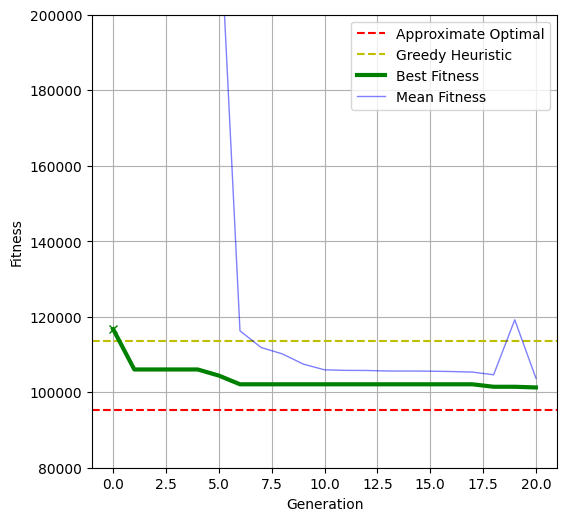
\includegraphics[width=0.5\textwidth]{results/4.5/tour929_convergence.png}
    \caption{Tour929 Convergence Graph}
    \label{fig:tour929convergence}
\end{figure}

\section{Critical reflection}

\RemoveMe{\textbf{Goal:} Based on this section, we will evaluate your understanding and insight into the main strengths and weaknesses of your evolutionary algorithms.}

\ReplaceMe{Describe the main lessons learned from this project. What do you think are the main strong points of evolutionary algorithms in general? Did you apply these strengths in this project? What are the main weaknesses of evolutionary algorithms and of your implementation in particular? Do you think these can be avoided or mitigated? How? Do you believe evolutionary algorithms are appropriate for this problem? Why (not)? What surprised you and why? What did you learn from this project?}

%\section{Other comments} \label{sec_other}
%
%\ReplaceMe{In case you think there is something important to discuss that is not covered by the previous sections, you can do it here. }

\bibliographystyle{plain}
\bibliography{ref}

\end{document}
